\documentclass[border=10pt]{standalone}
\usepackage{pgfplots}
\pgfplotsset{compat=1.18}
\begin{document}
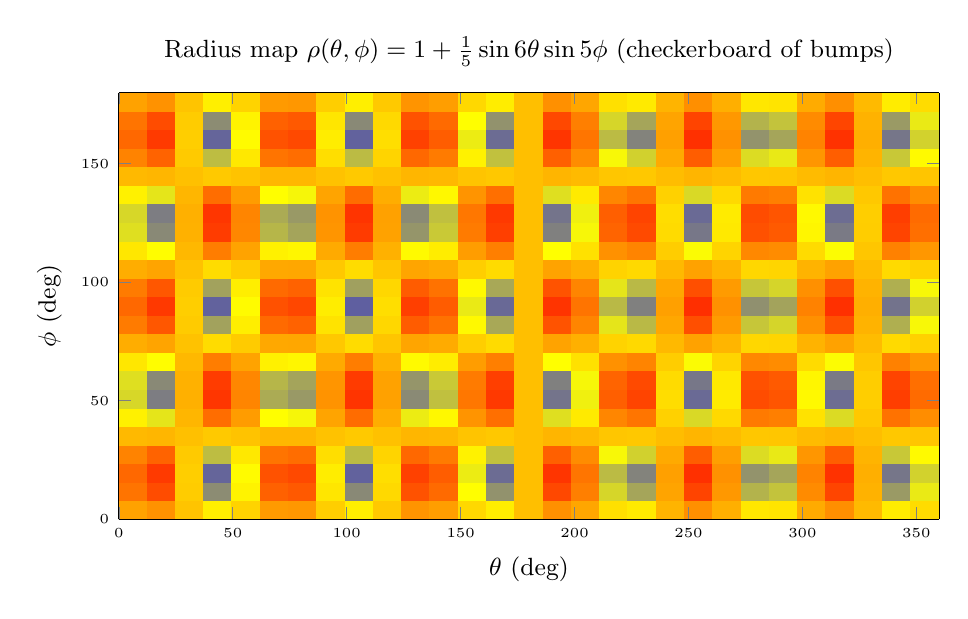
\begin{tikzpicture}
\begin{axis}[
    view={0}{90},
    domain=0:360, samples=30,
    y domain=0:180, samples y=24,
    width=12cm, height=7cm,
    tick label style={font=\tiny},
    label style={font=\small},
    title style={font=\small},
    xlabel={$\theta$ (deg)}, ylabel={$\phi$ (deg)},
    title={Radius map $\rho(\theta,\phi)=1+\frac{1}{5}\sin 6\theta\sin 5\phi$ (checkerboard of bumps)},
]
\addplot3[surf, shader=flat] { 1+0.2*sin(6*x)*sin(5*y) };
\end{axis}
\end{tikzpicture}
\end{document}